%%%%%%%%%%%%%%%%%%%%%%%%%%%%%%%%%%%%%%%%%
% University/School Laboratory Report
% LaTeX Template
% Version 3.0 (4/2/13)
%
% This template has been downloaded from:
% http://www.LaTeXTemplates.com
%
% Original author:
% Linux and Unix Users Group at Virginia Tech Wiki 
% (https://vtluug.org/wiki/Example_LaTeX_chem_lab_report)
%
% License:
% CC BY-NC-SA 3.0 (http://creativecommons.org/licenses/by-nc-sa/3.0/)
%
%%%%%%%%%%%%%%%%%%%%%%%%%%%%%%%%%%%%%%%%%

%----------------------------------------------------------------------------------------
%	PACKAGES AND DOCUMENT CONFIGURATIONS
%----------------------------------------------------------------------------------------

\documentclass{article}

\usepackage[version=3]{mhchem} % Package for chemical equation typesetting
\usepackage{siunitx} % Provides the \SI{}{} command for typesetting SI units

\usepackage[top=1in, bottom=1in, right=1in, left=1in]{geometry}

%Add code formating
\usepackage{listings}
\lstset{tabsize=2}

\usepackage{hyperref}

\usepackage{amssymb}

\usepackage{enumerate}

\usepackage{multicol} % Multi-column support

%Add extra support for image placement
\usepackage{float}

\usepackage{mcode}

\usepackage{graphicx} % Required for the inclusion of images

\setlength\parindent{0pt} % Removes all indentation from paragraphs

\renewcommand{\labelenumi}{\alph{enumi}.} % Make numbering in the enumerate environment by letter rather than number (e.g. section 6)

%\usepackage{times} % Uncomment to use the Times New Roman font

%----------------------------------------------------------------------------------------
%	DOCUMENT INFORMATION
%----------------------------------------------------------------------------------------

\title{Qt Widget Quick Start} % Title

\author{Blake \textsc{Vermeer}} % Author name

\date{\today} % Date for the report

\begin{document}

\maketitle % Insert the title, author and date

\begin{center}
\begin{tabular}{l r}
Date Performed: & April 3, 2017 \\ % Date the experiment was performed
Company: & Keysight Technologies % Company
\end{tabular}
\end{center}

% If you wish to include an abstract, uncomment the lines below
% \begin{abstract}
% Abstract text
% \end{abstract}

%----------------------------------------------------------------------------------------
%	OVERVIEW
%----------------------------------------------------------------------------------------
\section{Overview}

In this tutorial you will learn how to create a basic Qt Widget application from scratch and deploy it to the Keysight Hacking Platform development kit.



%----------------------------------------------------------------------------------------
%	Create a new Qt Widget Application Project
%----------------------------------------------------------------------------------------
\section{Creating a New Qt Widgets Project}

	\begin{enumerate}[1.)]
		\item First we will use Qt Creator's new project wizard to create a new Qt Widgets project template. First open Qt Creator and then go to \textbf{File $\rightarrow$ New File or Project...}
		
		\item The new project wizard dialog box will pull up. Make sure the \textbf{Generic Linux Device Templates} option is selected in the drop-down menu in the upper right. Select \textbf{Applications} from the left hand menu under projects and then select the \textbf{Qt Widgets Application} project template and then click the \textbf{Choose...} button.
		
			\begin{figure}[H]
				\centering
				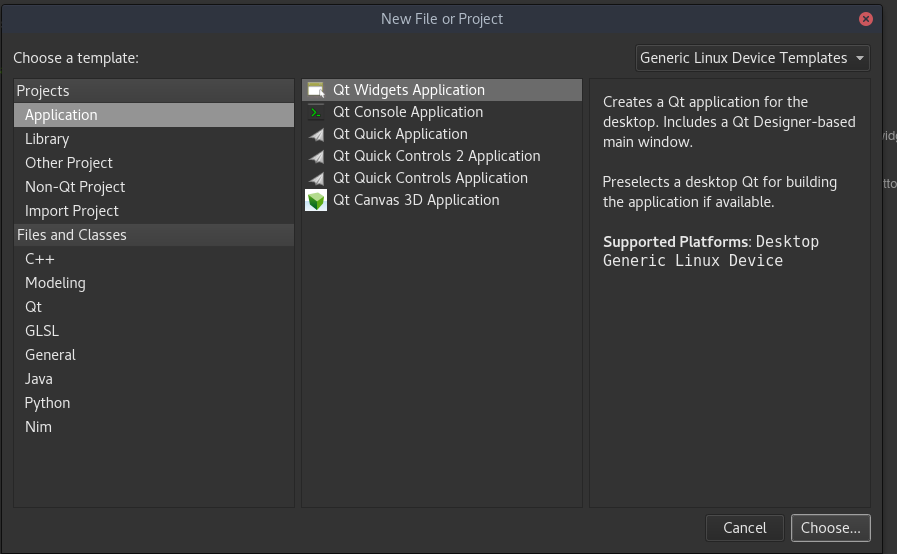
\includegraphics[width=0.85\textwidth]{pics/Choose_Project_Type.png}
				\caption{New Project Wizard Dialog Box}
				\label{Choose_Project_Type}
			\end{figure}
		
		\item In the next dialog box choose a name for the project and where to save it and then click the \textbf{Next} button.
		
			\begin{figure}[H]
				\centering
				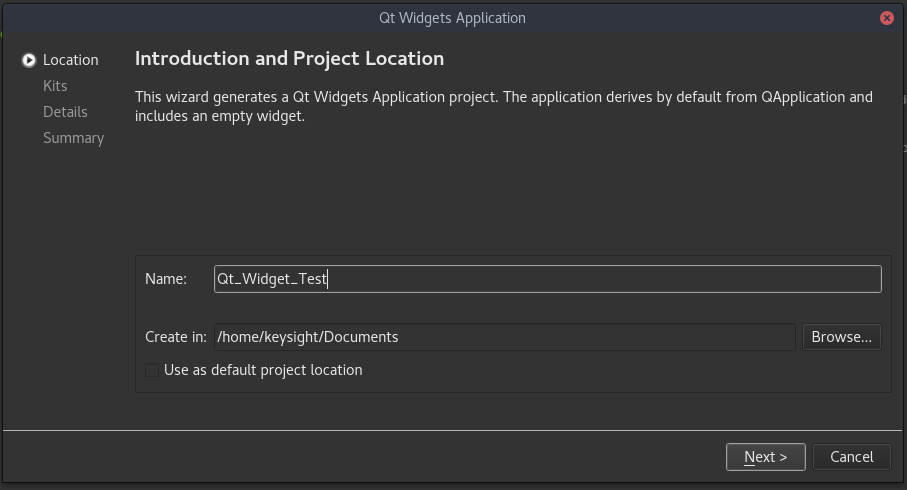
\includegraphics[width=0.85\textwidth]{pics/Name_Project.png}
				\caption{Name the Project}
				\label{Name_Project}
			\end{figure}
		
		\item In the next dialog box make sure that only the \textbf{RPi} box is selected since we are not trying to build a desktop application and then click the \textbf{Next} button.
		
			\begin{figure}[H]
				\centering
				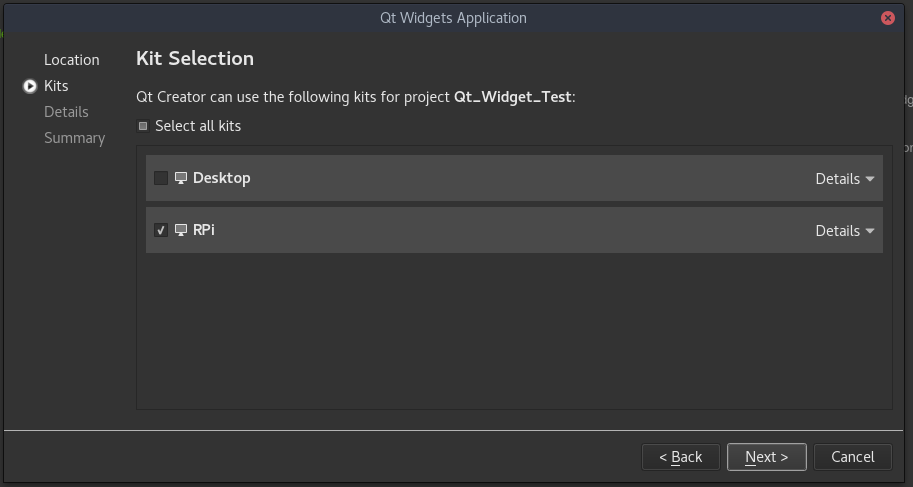
\includegraphics[width=0.85\textwidth]{pics/Kit_Selection.png}
				\caption{Kit Selection}
				\label{Kit_Selection}
			\end{figure}	
		
		\item In the \textbf{Class Information} dialog box leave everything at their default values and click the \textbf{Next} button.
		
			\begin{figure}[H]
				\centering
				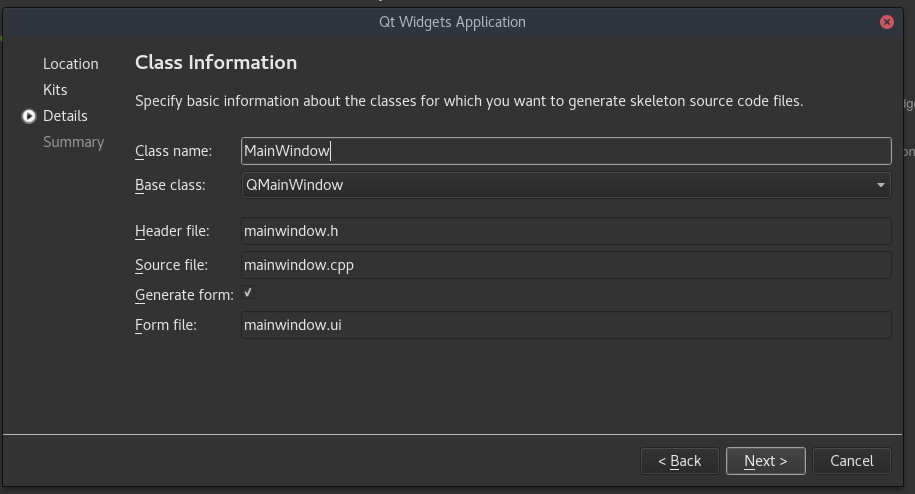
\includegraphics[width=0.85\textwidth]{pics/Class_Info.png}
				\caption{Class Information}
				\label{Class_Info}
			\end{figure}		
		
		\item In the \textbf{Project Management} dialog box leave everything alone and click the \textbf{Finish} button.
		
			\begin{figure}[H]
				\centering
				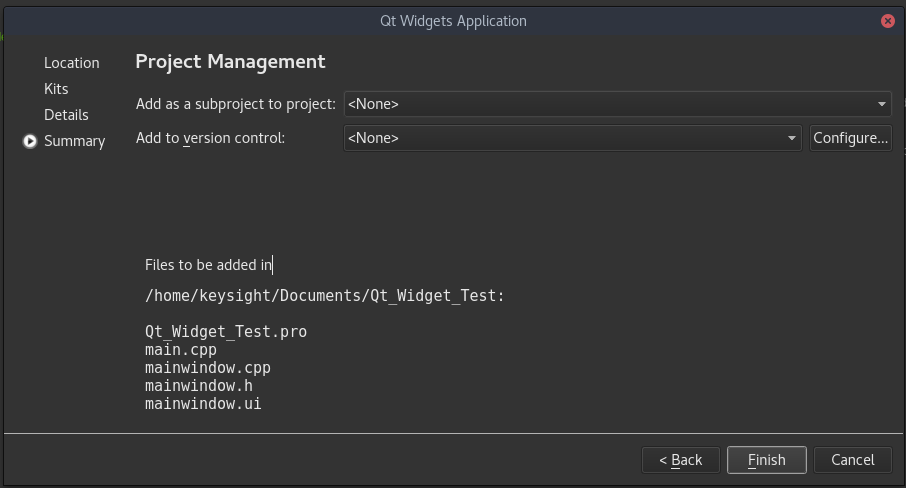
\includegraphics[width=0.85\textwidth]{pics/Project_Management.png}
				\caption{Project Management}
				\label{Project_Management}
			\end{figure}		
		
	\end{enumerate}


%----------------------------------------------------------------------------------------
%	Qt Widgets Project Overview
%----------------------------------------------------------------------------------------
\section{Qt Widgets Project Overview}

The Qt Widgets project wizard creates several different files. This section gives a brief overview of the files created and their purpose.


	\begin{figure}[H]
		\centering
		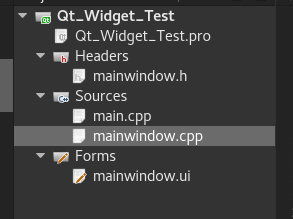
\includegraphics[width=0.25\textwidth]{pics/Project_Files.png}
		\caption{Project Files Created for a Project Name "Qt\_Widget\_Test"}
		\label{Project_Files}
	\end{figure}


Here is a brief overview of the files created for a project called Qt\_Widget\_Test and their purpose:

\begin{itemize}
	\item \textbf{Qt\_Widget\_Test.pro} - The main project file. The project file defines the source files used by the project, the name of the application, where to deploy the application on the target device, and various other settings.
	
	\item \textbf{mainwindow.h} - A header file for the \textit{mainwindow} class. 
	
	\item \textbf{main.cpp} - The main source file for the application. It creates a \textit{QApplication} object need for Qt Widget programs and then creates a \textit{mainwindow} object and displays it.
	
	\item \textbf{mainwindow.cpp} - The source file for the \textit{mainwindow} class. This class inherits from \textit{Q\_OBJECT} and defines the actions done by the various \textit{mainwindow} GUI events.
	
	\item \textbf{mainwindow.ui} - The UI for for the \textit{mainwindow widget}. This file defines the GUI layout for the application.
\end{itemize}


%----------------------------------------------------------------------------------------
%	Preparing the Project File
%----------------------------------------------------------------------------------------
\section{Preparing the Project File}

The default created project file is almost fully complete. The only thing that needs to be added is a target path definition that will tell Qt Creator where to install the application on the target device when deploying it. Add the three lines as shown in Figure \ref{Target_Path}.

	\begin{figure}[H]
		\centering
		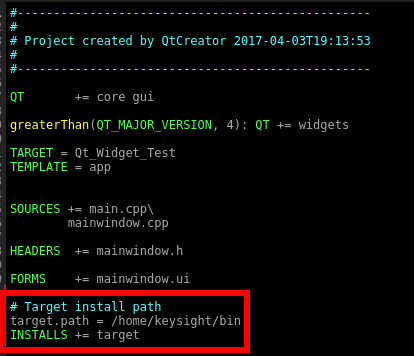
\includegraphics[width=0.5\textwidth]{pics/Add_Target.png}
		\caption{Define the target install path}
		\label{Target_Path}
	\end{figure}


%----------------------------------------------------------------------------------------
%	Creating the GUI
%----------------------------------------------------------------------------------------
\section{Creating the GUI}

This section will explain how to main a basic GUI. Double-click the \textit{mainwindow.ui} file. It will automatically open in the design view.





%----------------------------------------------------------------------------------------
%	APPENDIX
%----------------------------------------------------------------------------------------

%\newpage
%\section{Appendix}

%\begin{enumerate}

	
%	\item[1. a.)] \lstinputlisting{../MATLAB/problem_1a.m}
	

%\end{enumerate}






%----------------------------------------------------------------------------------------


\end{document}